% Intended LaTeX compiler: pdflatex
\documentclass[10pt,a4paper,UTF8]{article}
\usepackage{zclorg}
\author{zcl.space}
\date{}
\title{排列组合分析}
\hypersetup{
 pdfauthor={zcl.space},
 pdftitle={排列组合分析},
 pdfkeywords={probability},
 pdfsubject={本文介绍概率论中最基本的数数规则},
 pdfcreator={Emacs 25.0.50.1 (Org mode 9.0.6)},
 pdflang={English}}
\begin{document}

\maketitle
\tableofcontents
\titlepic{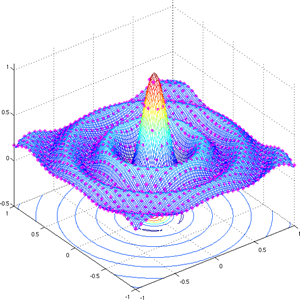
\includegraphics[scale=0.25]{../../img/sinc.PNG}}
本文介绍最简单的数数规则,这类的概率问题可难也可简单。我记得上高中的时候比较麻烦的一个问题是两盒火柴的问题,大意如下:两个火柴盒里面放火柴,然后随机抽取,问第\(n\)次以后恰好第一个盒子的火柴被抽光的概率。这类的问题需要掌握一些基本的规则,按照规则逐步计算会容易的多。


\textbf{计数基本法则} 如果一共有\(r\)个试验,试验\(1\)有\(n_{1}\)中结果,对于试验\(1\)的每一种可能,试验\(2\)都有\(n_{2}\)中结果,对于前两个试验的每一种可能的结果,试验\(3\)都有\(n_{3}\)种结果,依次类推,这\(r\)个试验一共有\(n_{1}n_{2}\ldots n_{r}\)种结果。

\textbf{排列} 假设有\(n\)个互不相同的元素,则一共有\(n!\)个排列结果。如果这\(n\)个元素,其中\(n_{1}\)个彼此相同,另\(n_{2}\)个彼此相同,依次类推,\(n_{r}\)个也彼此相同,那么一共排列的个数为:
\begin{equation}
\label{eq:1}
\frac{n!}{n_{1}!n_{2}!\ldots n_{r}!}
\end{equation}

\textbf{组合} 一般来说,如果考虑顺序,从\(n\)个元素中取出\(r\)个排成一组,一共有\(n(n-1)\ldots (n-r+1)\)种不同的方式,而每个包含\(r\)个元素的小组都被重复计算了\(r!\)次。所以从\(n\)个元素中取出\(r\)个组成不同组的数目为:
\begin{equation}
\label{eq:2}
\frac{n(n-1)\ldots (n-r+1)}{r!} = \frac{n!}{(n-r)!r!}
\end{equation}
因此,如果不考虑顺序, \(\binom{n}{r}\)表示从\(n\)个元素中取出\(r\)个元素所组成的不同组的数目。

\begin{instance}
假设在一排\(n\)个天线中,有\(m\)个是失效的,另\(n-m\)个时有效的。假设所有有效天线不可区分,所有失效的天线之间也不可区分。为有多少中线性排列方式,使得任何两个失效的天线都不相邻?
\end{instance}

\begin{answer}
把\(n-m\)个有效天线排一排。既然不允许连续两个失效天线在一起,那么这两个有效天线之间必然至多放置 一个失效的。即在\(n-m+1\)的位置中选择\(m\)个来放置,因此有\(\binom{n-m+1}{m}\)种放置方法。
\end{answer}

一个非常有用的组合恒等式:
\begin{equation}
\label{eq:3}
\binom{n}{r} = \binom{n-1}{r-1} + \binom{n-1}{r}
\end{equation}
这个式子的证明可以从分析的角度来证明,也可以从组合的角度来证明。当然,从组合的角度来证明更能显示出这个式子的意义。设想从\(n\)个元素中取\(r\)个,一共有\(\binom{n}{r}\)种取法。从另一个角度来考虑,不妨假设这\(n\)个元素里有一个特殊的,记为元素\(1\),那么取\(r\)个元素就有两种结果:取元素\(1\)或者不取\(1\)。取元素\(1\)时,一共有\(\binom{n-1}{r-1}\)中方法;不取元素\(1\)时,一共有\(\binom{n-1}{r}\)。两者之和就是从\(n\)个元素里取\(r\)个的方法直和,而从\(n\)个元素中取\(r\)个共有\(\binom{n}{r}\)。

\(\binom{n}{r}\)经常成为二项式系数,因为他们是二项式定理中重要的系数。接下来用两种方法证明二项式定理

\begin{theorem}
\begin{equation}
\label{eq:4}
(x+y)^{n} = \sum_{k=0}^{n}\binom{n}{k}x^{k}y^{n-k}
\end{equation}
\end{theorem}
\begin{proof}
首先我们用数学归纳法来证明。

当\(n=1\)时,\(x+y = \binom{1}{0}x^{0}y^{1} + \binom{1}{1}x^{1}y^{0} = y+x\)
假设式 (\ref{eq:4}) 对于\(n-1\)成立,那么对于\(n\):
\begin{eqnarray}
\label{eq:5}
(x+y)^{n}&=& (x+y)^{n-1}(x+y) \\
&=& \sum_{i=0}^{n-1}\binom{n-1}{i}x^{i}y^{n-1-i}(x+y) \\
&=& \sum_{i=0}^{n-1}\binom{n-1}{i}x^{i+1}y^{n-1-i}  + \sum_{i=0}^{n-1}\binom{n-1}{i}x^{i}y^{n-i}
\end{eqnarray}
对于上式右端第一项令\(k = 1 + i\),右端第二项令\(i=k\),则:
\begin{eqnarray}
\label{eq:6}
(x+y)^{n}&=& \sum_{i=0}^{n-1}\binom{n-1}{i}x^{i+1}y^{n-1-i}  + \sum_{i=0}^{n-1}\binom{n-1}{i}x^{i}y^{n-i}  \\
&=& \sum_{k=1}^{n} \binom{n-1}{k-1}x^{k}y^{n-k} + \sum_{k=0}^{n-1}\binom{n-1}{k}x^{k}y^{n-k} \\
&=& x^{n} + \sum_{k=1}^{n-1} \binom{n-1}{k-1}x^{k}y^{n-k} + \sum_{k=1}^{n-1}\binom{n-1}{k}x^{k}y^{n-k} + y^{n} \\
&=& x^{n} + \sum_{k=1}^{n-1} \bigg( \binom{n-1}{k-1} + \binom{n-1}{k} \bigg)x^{k}y^{n-k} + y^{n} \\
&=& x^{n} + \sum_{k=1}^{n-1} \binom{n}{k} x^{k}y^{n-k} + y^{n} \\
&=& \sum_{k=0}^{n} \binom{n}{k}x^{k}y^{n-k}
\end{eqnarray}
\end{proof}

\begin{proof}
接下来给出另外一种证明方法。考虑乘积:
\begin{equation}
\label{eq:7}
(x_{1} + y_{1})\ldots  (x_{n} + y_{n})
\end{equation}
它展开后包括\(2^{n}\)个求和项,每一项都是\(n\)个因子的乘积,而且每一项都包含因子\(x_{i}\)或者\(y_{i}\),\(i=1,\ldots ,n\),例如:
\[(x_{1} + y_{1})(x_{2} + y_{2}) = x_{1}x_{2} + x_{1}y_{2} + y_{1}x_{2} + y_{1}y_{2}\]
这\(2^{n}\)个求和项中,一共有多少项含有\(k\)个\(x\)相关的因子,多少项含有\(n-k\)个\(y\)相关的因子? 含有\(k\)个\(x\)相关因子和\(n-k\)个\(y\)相关因子的每一项对应从\(n\)个元素\(x_{1},\ldots ,x_{n}\)取\(k\)个元素组成一组的取法,因此一共有\(\binom{n}{k}\)中取法。这样令\(x_{i} = x,y_{i} = y,i=i,\ldots ,n\),可以看出:
\begin{equation}
\label{eq:8}
(x+y)^{n} = \sum_{k=0}^{n}\binom{n}{k}x^{k}y^{n-k}
\end{equation}
\end{proof}

\begin{instance}
一个含有\(n\)个元素的集合一共有多少子集?
\end{instance}
\begin{answer}
第一种解法:含有\(k\)个元素的集合一共有\(\binom{n}{k}\)个,因此所求答案是:\[\sum_{k=0}^{n}\binom{n}{k} = (1+1)^{n} = 2^{n}\]
第二种解法:把这\(n\)个元素排成一排,对于某个元素,可以包含于一个集合也可以不包含于这个集合。包含于某集合记为1,不包含于该集合记为0,则这样互不相同的二进制序列一共有\(2^{n}\)个。其对应了这\(n\)个元素的\(2^{n}\)个子集。
\end{answer}
\end{document}